\chapter{Metodologia i narzędzia uczenia maszynowego środowiska .NET}

Celem tej pracy jest wykorzystanie technologii uczenia maszynowego w środowisku .NET w celu detekcji choroby Alzheimera.
W tym rozdziale więc zostaną przedstawione narzędzia, które pomogą w osiągnięciu tego celu, w tym technologie uczenia maszynowego oraz sama platforma .NET.

\section{Technologie głębokiego uczenia maszynowego}

Teoretyczne zagadnienia związanie z technologiami głębokiego uczenia maszynowego, w szczególności głębokich konwolucyjnych sieci neuronowych zostały już omówione w \hyperref[sec:deep-learning]{sekcji \ref*{sec:deep-learning}}.
W tym rozdziale zostanie przedstawione w jaki sposób obiecująca teoria jest przekładana na wykorzystanie w praktyce.

\subsection{Symulator SNNS}

Tematykę oprogramowania służącego do tworzenia i trenowania sieci neuronowych warto zacząć omówienia przestarzałego już programu \emph{SNNS} (ang. Stuttgart Neural Network Simulator).
Pozwala on na tworzenie i trenowanie sieci neuronowych, a także -- co ważne przy jego zastosowaniach -- na ich wizualizację.

SNNS to program okienkowy napisany w języku C, przeznaczony głównie dla systemów Unixowych.
W ramach jego działania można zamodelować sieć neuronową po jednym neuronie, łącząc je z dużą dozą swobody w dowolne struktury oraz parametryzując je w dowolny sposób.
Następnie można zdefiniować zbiór danych uczących, a także zbiór danych testowych, na których można przeprowadzić proces uczenia sieci.

Całe tworzenie sieci jest czynnością bardzo czasochłonną i złożoną ze względu na manualną naturę definiowania jej struktury.
Daje za to bardzo dużo możliwości modyfikacji, w tym zmianę na przykład funkcji aktywacji pojedynczego neuronu, zachowania się konkretnego połączenia oraz wielu innych właściwości, które posiadają wszystkie obiekty możliwe do edycji w programie.

Najważniejszą cechą SNNS jest wizualny sposób budowy sieci neuronowej oraz manualny proces jej konfiguracji.
Nie jest ona może wtedy wystarczająco wydajna do jakichkolwiek problemów, z którymi potrafią radzić sobie nowoczesne sieci neuronowe, ale pozwala na zrozumienie ich działania oraz nauczenie się podstawowych zasad ich budowy.
Dlatego też mimo, iż sam program jest już przestarzały i wycofany z użytku a sami jego autorzy polecają użycie nowoczesnych bibliotek uczenia maszynowego takich jak TensorFlow czy PyTorch \cite{snns}, to nadal jest bardzo często wykorzystywany w celach edukacyjnych.

Pomimo, iż znane są metody znacznie przyspieszające działanie i uczenie sieci neuronowych przez reprezentacje wag i aktywacji jako macierzy i wektorów i ich późniejsze mnożenie przy pomocy zrównoleglonych obliczeń na kartach graficznych i dedykowanych urządzeniach, to założenia podstaw działania sztucznych sieci neuronowych pozostają niezmienne i programy typu SNNS pozwalają na znacznie prostsze ich poznanie i zrozumienie.

\subsection{Azure Machine Learning Studio}

\emph{Microsoft Azure Machine Learning Studio} (w skrócie \emph{AML Studio}) to kompleksowa platforma, która wykorzystywana jest do implementacji i zarządzania procesami uczenia maszynowego.
AML Studio oferuje zaawansowane narzędzia do tworzenia, wdrażania oraz monitorowania modeli uczenia maszynowego, integrując różnorodne etapy tego procesu w jednym środowisku.

Jest to platforma oparta na chmurze i posiadająca interfejs graficzny w postaci intuicyjnej strony internetowej, na której modelowanie przetwarzania danych i procesu uczenia odbywa się przy użyciu przeciągania i upuszczania elementów blokowych oraz łączenia ich w odpowiedni sposób.
Pozwala na tworzenie tak zwanych \emph{eksperymentów}, które składają się z kolejnych kroków w analizie danych i tworzeniu modeli.
Dzięki temu możliwe jest systematyczne badanie różnych podejść i łatwe porównywanie ich wyników.
Graficzny sposób reprezentacji wykorzystanych modułów w eksperymencie a także przepływu danych między nimi pozwala na uproszczenie wyszukiwania potencjalnych błędów lub problemów pojawiających się w całym procesie.
Możliwe jest również analizowanie w czasie rzeczywistym działania modelu i analizę przez niego danych w całym eksperymencie.

Bardzo istotną cechą AML Studio jest fakt, że platforma integruje się z innymi usługami chmurowymi dostarczanymi przez Microsoft Azure, co umożliwia tworzenie spójnych rozwiązań opartych na chmurze.
Pozwala na dynamiczne wczytywanie danych z innych źródeł znajdujących się w chmurze, a także na wdrażanie modeli uczenia maszynowego w postaci usług sieci Web, które mogą być wykorzystywane przez inne aplikacje.

Wykorzystanie Azure Machine Learning Studio dzięki swoim cechom pozwala na szybki trening modelu uczenia maszynowego oraz jego wdrożenie bez konieczności pisania kodu czy głębszej znajomości tematyki uczenia maszynowego \cite{mukunthu2019practical}, w szczególności gdy z założenia wdrożony model ma działać w chmurze i integrować się z innymi systemami w niej obecnymi.
Jednak w zastosowaniach, które nie czerpią korzyści z połączenia z chmurą i dają swobodę czasową na własnoręczne zaimplementowanie modelu, wykorzystanie AML Studio może być nieopłacalne ze względu na koszty związane z jego wykorzystaniem w większych ilościach.
Warto wtedy rozważyć inne rozwiązania, które dają swobodę konstruowania i trenowania modelu od podstawi i dostrojenie go do bardziej złożonych zadań, maksymalizując tym samym osiągane możliwości i dokładność -- a są to zazwyczaj biblioteki uczenia maszynowego w językach programowania.

\subsection{TensorFlow i Keras}
\label{sec:tensorflow-and-keras}

Jedną z najpopularniejszych bibliotek uczenia maszynowego, która jest wykorzystywana do tworzenia i trenowania sieci neuronowych jest \emph{TensorFlow}.
Jest to otwartoźródłowa platforma do obliczeń numerycznych i implementacji modeli uczenia maszynowego.
Jego fundamentem jest reprezentacja danych w postaci tensorów, co umożliwia wykonywanie skomplikowanych operacji matematycznych na dużych zbiorach danych \cite{shukla2018machine}.

TensorFlow jest bilbioteką niskopoziomową napisaną głównie w języku C++ i implementującą często używane algorytmy uczenia maszynowego i sieci neuronowych i wystawiającą je jako interfejs programistyczny w językach wyższego poziomu takich jak Python czy JavaScript.
Napisany został pierwotnie przez zespół badawczy Google Brain.

Jednak ze względu swoje dążenie do umożliwienia jak największej elastyczności i kontroli nad procesem uczenia sieci neuronowych, TensorFlow w swojej czystej postaci wymaga od programisty dużo pracy i wiedzy, aby zaimplementować nawet najprostszy model sieci neuronowej.

W celu uproszczenia z korzystania z TensorFlow powstały ``frontendy'' dla różnych języków programowania pozwalające na wykorzystanie jego możliwości w bardziej przyjazny sposób.
Jednym z nich jest \emph{Keras}, który jest wysokopoziomowym interfejsem programistycznym dla TensorFlow w języku Python.
Jest to jeden z najpopularniejszych interfejsów programistycznych dla TensorFlow ze względu na swoją prostotę i intuicyjność.

Dla uproszczenia wystawia API sekwencyjne (ang. Sequential API), które przez wykorzystanie istniejących klas i ``sekwencyjne'' tworzenie obiektów symbolizujących określone rodzaje warstw ze zdefiniowanymi odpowiednio parametrami pozwala na proste w śledzeniu i zrozumieniu stworzenie struktury sieci neuronowych.
Operacje takie jak \emph{skompilowanie} (czyli utworzenie z definicji warstw sieci zoptymalizowanego do uruchomienia i uczenia wstępnego modelu) definicji modelu używając odpowiednich parametrów czy uruchomienie trenowania (ang. \emph{fit}) w odpowiedniej konfiguracji wykonuje się wywołaniem tylko  jednej metody.

Mimo swojej prostoty, Keras pozwala na również na podejścia bardziej eksperckie.
W nich oprócz definiowania sekwencyjnego struktury sieci można również tworzyć własne klasy reprezentujące niestandardowe warstwy lub całe bloki odpowiednio ustrukturyzowane i zparametryzowane.

Uczenie sieci neuronowej w Keras zachowuje również zbiór metryk, które pozwalają na prześledzenie postępów w procesie uczenia i wykorzystanie ich do analizy lub optymalizacji modelu albo całego schematu programu.

Sukces TensorFlow oraz Keras wynika głównie z połączenia ich wydajności, elastyczności i prostoty użycia, które w dużej mierze są zasługą również wykorzystanego języka programowania Python, najpopularniejszego do zastosowań w uczeniu maszynownym.
Jednak ze względu na to, że obie te biblioteki mają swoje źródła dostępne na bazie licencji Apache 2.0 w publicznie dostępnym repozytorium serwisu GitHub \cite{tensorflow}.
Pozwala to społeczności na własne próby rozszerzenia zasięgu platformy do innych języków programowania, na przykład jak zostanie opisane w rozdziale \hyperref[sec:tensorflownet]{rozdziale \ref*{sec:tensorflownet}} -- do języka C\#.

\section{Platforma .NET}

Platforma .NET jest kompleksowym środowiskiem programistycznym opracowanym przez pierwotnie firmę Microsoft, a obecnie rozwijanym przez niezależną organizację non-profit \emph{.NET Foundation} oraz społeczność programistów.

W celu lepszego zrozumienia aktualnego stanu platformy warto przyjrzeć się jej historii i poprzednikowi, którym jest \emph{.NET Framework}.
Jest to starsza wersja, która była szeroko wykorzystywana przed pojawieniem się \emph{.NET Core} (i nadal jest w wielu przestarzałych bazach kodu określanych jako \emph{legacy code}).
Działała ona wyłącznie na systemach operacyjnych Windows i była bardzo ściśle z nimi związana.
Miał bardzo szerokie zastosowania, pozwalał na pisanie aplikacji okienkowych, konsolowych, usług systemowych czy aplikacji sieciowych z użyciem różnych języków programowania -- głównie najpopularniejszego obiektowego języka C\#, ale także Visual Basic czy funkcjonalnego F\#.
\emph{.NET Framework} został wypuszczony w 2002 jako konkurent dla platformy Java i jej maszyny wirtualnej JVM, która również pozwala na pisanie aplikacji w wielu językach programowania i jest niezależna od systemu operacyjnego.
Podobnie jak ona kod kompilowany jest do kodu pośredniego, który jest wykonywany przez maszynę wirtualną \emph{Common Language Runtime} (CLR) -- odpowiednika JVM w Javie.
Kod ten nazywa się \emph{IL} (ang. \emph{Intermediate Language}, odpowiednik \emph{Java bytecode}) i jest zapisywany w plikach o rozszerzeniu \emph{.dll} (ang. \emph{Dynamic Link Library}) lub \emph{.exe} (ang. \emph{Executable})
Tak skompilowany kod jest później uruchamiany przez interpreter CLR, podobnie jak ma to miejsce w przypadku JVM (\emph{Java Virtual Machine}).

W 2014 roku Microsoft ogłosił, że rozpoczyna prace nad nową wersją platformy .NET, którego rozwój ma odbywać się pod nadzorem nowej, niezależnej organizacji non-profit \emph{.NET Foundation}.
Wersja stabilna 1.0 nowego tworu nazwanego \emph{.NET Core} została wydana w 2016 roku jako platforma w pełni otwartoźródłowa, międzyplatformowa i modułowa.
Oznacza to, że jest ona dostępna na systemach operacyjnych Windows, Linux i macOS, a także że jej komponenty są dostępne jako osobne pakiety, które można wykorzystywać w zależności od potrzeb.
Cały kod źródłowy jest dostępny już na portalu GitHub, upubliczniony z bardzo liberalną licencją MIT \cite{dotnet-sdk-repo, dotnet-runtime-repo}, wraz ze wszystkimi bibliotekami wbudowanymi służącymi do tworzenia różnych rodzajów oprogramowania, a nawet repozytorium służące do rozwijania składni języka wraz z wkładem od społeczności.
Od tamtego czasu nowa wersja platformy poza jednym wyjątkiem była wypuszczana co roku.
W 2020 roku, po poprzednim wydaniu .NET Core 3.1 ogłoszono, że pominięta zostanie wersja 4 ze względu na możliwe mylenie jej z działającą wtedy jeszcze w wielu miejscach wersją 4.8 starszego \emph{.NET Framework}.
Dodatkowo celu unifikacji nazewnictwa oraz sprostowanie, że .NET Core nie jest okrojoną wersją ale pełnoprawną platformą, która jako jedyna będzie dalej rozwijana, zdecydowano się na pomięcie członu \emph{Core} i od wersji 5.0 platforma nazywa się po prostu \emph{.NET 5}.

\subsection{Język C\#}

Język programowania C\# jest jednym z najpopularniejszych języków programowania na platformie .NET.

Jest to język obiektowy, który został zaprojektowany przez Microsoft w 2000 roku jako główny język platformy .NET.
Od tego czasu jest stale rozwijany i wraz z nowymi wersjami platformy .NET pojawiają się nowe wersje języka C\#, z najnowszą na moment pisania niniejszej pracy wersją \emph{C\# 11} wypuszczoną razem z \emph{.NET 7} w 2022 roku.
Rozwój języka przebiega wraz ze wkładem społeczności, która zgłasza propozycje nowych funkcjonalności i poprawek do istniejących przy użyciu oficjalnego repozytorium języka na portalu GitHub \cite{dotnet-csharplang-repo}, na którym dodatkowo znajduje się historia wszystkich proponowanych zmian oraz informacje na ich temat, a także notatki z wewnętrznych spotkań \emph{.NET Foundation} dotyczących dalszego projektu języka.

Kilka cech języka:

\begin{itemize}

  \item Bezpieczeństwo typów: C\# jest językiem silnie typowanym, co oznacza, że typy zmiennych są sprawdzane podczas kompilacji, co pomaga uniknąć wielu błędów w czasie działania programu.

  \item Automatyczne zarządzanie pamięcią:Automatyczne zarządzanie pamięcią: Dzięki mechanizmom takim jak Garbage Collection (zbieranie nieużywanej pamięci) C\# pozwala programistom uniknąć wielu problemów związanych z wyciekami pamięci.

  \item Asynchroniczność: C\# oferuje obszerną obsługę operacji asynchronicznych, co jest szczególnie ważne w aplikacjach wielowątkowych i sieciowych.

\end{itemize}

Dodatkowo język ten jest bardzo elastyczny i pozwala na wykorzystanie wielu paradygmatów programowania, w tym obiektowego, imperatywnego, funkcyjnego czy generycznego.
W szczególności ostatni rozwój języka brnie w kierunku paradygmatu funkcyjnego inspirowany językami takimi jak F\# -- również z rodziny \emph{.NET} -- czy Haskell.
Jednym z przykładów jest rosnąca popularność użycia ``fluent interfejsów'', czyli pisania metod w taki sposób, by pozwalały na ich łańcuchowe wywoływanie, co pozwala na pisanie kodu w sposób bardzo czytelny.

Przykładowo poniższy fragment kodu z projektu \lstinline{MLModel_ConsoleApp} napisanego w dodatku do tej pracy pozwala na zbudowanie potoku przetwarzania danych, który składa się z trzech kroków poprzez proste wywoływanie metod po sobie na własnych zwracanych obiektach.

\begin{lstlisting}[language={[Sharp]C}]
public static IEstimator<ITransformer> BuildPipeline(MLContext mlContext)
{
    // Data process configuration with pipeline data transformations
    var pipeline = mlContext.Transforms.Conversion.MapValueToKey(/*...*/)
        .Append(mlContext.MulticlassClassification.Trainers.ImageClassification(/*...*/))
        .Append(mlContext.Transforms.Conversion.MapKeyToValue(/*...*/));

    return pipeline;
}
\end{lstlisting}

W ten sposób kod jest czytelny i łatwy do zrozumienia, a dodatkowo pozwala na łatwe dodawanie kolejnych kroków do potoku bez konieczności dużej zmiany istniejącego kodu.
Jest to szczególnie przydatne do implementacji wzorców projektowych takich jak \emph{Builder} czy \emph{Decorator}, które w C\# są wykorzystywane bardzo często.

\subsection{Język F\#}

F\# jest językiem funkcyjnym, co oznacza, że skupia się na programowaniu funkcyjnym, w którym funkcje są traktowane jako podstawowe jednostki programu
Funkcje w F\# są traktowane jak wartości, co umożliwia bardziej zdeklarowane i modularne podejście do programowania.

Najważniejsze cechy języka:

\begin{itemize}

  \item Kompaktowość: Funkcyjny styl programowania często pozwala na bardziej zwięzły kod w porównaniu do tradycyjnych języków.

  \item Bezpieczeństwo typów: F\# jest językiem silnie typowanym, co pomaga w unikaniu błędów podczas kompilacji i działania programu.

  \item Współbieżność: Dzięki naturze funkcyjnej, F\# ma wbudowane mechanizmy ułatwiające programowanie współbieżne i równoległe.

  \item Pattern matching: Jest to potężna technika w F\#, która pozwala na efektywne przetwarzanie i rozpoznawanie różnych wzorców w danych.

\end{itemize}

F\# przynależy on do rodziny języków \emph{.NET}, przez co jest w pełni kompatybilny z pozostałymi językami i kompilowany jest do tego samego kodu \emph{IL} i można go wykorzystywać w taki sam sposób jak inne języki z tej rodziny, a paczki napisane w F\# mogą być wykorzystywane przez inne języki i na odwrót.
Dla przykładu w projekcie \lstinline{MLNetCustom} napisanym do tej pracy napisałem bibliotekę \lstinline{Plot} w języku F\#, ponieważ sekwencyjne tworzenie wykresów bardzo pasowało do funkcyjnego paradygmatu programowania.
Następnie bibliotekę tę wykorzystałem w głównym projekcie napisanym w języku C\# bez żadnych problemów z kompatybilnością.

\section{Framework uczenia maszynowego ML.NET}

\emph{ML.NET} to otwartoźródłowy i międzyplatformowy framework uczenia maszynowego dla platformy .NET.
Repozytorium z jego kodem źródłowym jest publiczne i udostępnione na portalu GitHub z licencją MIT \cite{dotnet-machinelearning-repo}.
Umożliwia programistom tworzenie modeli uczenia maszynowego w języku C\# lub F\# bez konieczności głębokiego zrozumienia matematyki lub statystyki.
Jest to narzędzie skierowane do programistów platformy .NET chcących wykorzystać uczenie maszynowe w swoich projektach bez potrzeby nauki innych języków programowania lub korzystania z zewnętrznych narzędzi.

Ważnym aspektem, który warto podkreślić, jest integracja ML.NET z istniejącą infrastrukturą .NET.
Pozwala to wykorzystać dostępne w .NET narzędzia i biblioteki do wczytywania danych, przetwarzania, wizualizacji i zarządzania modelem.
To sprawia, że praca z danymi i modelami jest bardziej spójna i efektywna.

ML.NET dostarcza zestaw gotowych algorytmów uczenia maszynowego, takich jak klasyfikacja, regresja, klasteryzacja, przetwarzanie języka naturalnego i wiele innych.
Można wybrać odpowiedni algorytm do swojego zadania bez konieczności implementowania go od zera.
Ważne spostrzeżenie tutaj to fakt, że ten zestaw daje odgórny podział na kategoria zadań do wykonania.
Nie pozwala na przykład zbudować warstwa po warstwie modelu głębokiej sieci neuronowej.
Zamiast tego wystawia klasy takie jak \lstinline{MulticlassClassification} dającą dostęp do zbioru już zaimplementowanych narzędzi i algorytmów klasyfikacji wieloklasowej, lub \lstinline{ImageClassificationTrainer} pozwalający na trenowanie modelu klasyfikacji obrazów.
Konfiguracja tego drugiego opiera się wyłącznie na zdefiniowaniu informacji dotyczących danych i hiperparametrów uczenia, takich jak wielkość paczki danych (ang. batch size), liczba epok (ang. epochs), czy współczynnik uczenia (ang. learning rate).
Dodatkowo można ustawić w jaki sposób współczynnik uczenia ma się zmieniać z czasem (ang. learning rate scheduler lub learning rate decay), czy testowanie powinno odbywać się także na zbiorze uczącym, kryteria zatrzymania uczenia (ang. early stopping criteria) czy metodę callbackową (ang. callback method), która zostanie wywołana po każdej epoce uczenia.

Jedna z istotniejszych opcji konfiguracji obiektu \lstinline{ImageClassificationTrainer} to wybór architektury, na której bazie będzie przeprowadzane uczenie.
Jest tak dlatego, ponieważ klasyfikacja obrazów ML.NET działa na podstawie uczenia transferowego omówionego od strony teoretycznej w sekcji \hyperref[sec:transfer-learning]{sekcji \ref*{sec:transfer-learning}}.
Dostępne do wybrania architektury to \emph{InceptionV3}, \emph{MobilenetV2}, \emph{ResnetV250} oraz domyślna \emph{ResnetV2101}.
Takie podejście pozwala na szybkie zbudowanie modelu uczenia maszynowego bez konieczności głębokiego zrozumienia jego działania, skupiając się wyłącznie na oczekiwanym celu.

W ramach mojego badania jeden z projektów jest oparty o czy ML.NET budowany kodowo -- solucja \lstinline{MLNetCustom}.
Jednak ML.NET można wykorzystać także bez bezpośredniego pisania kodu dotyczącego modelu i uczenia z użyciem rozszerzenia do Visual Studio \emph{ML.NET Model Builder}.

\subsection{ML.NET Model Builder}

\emph{ML.NET Model Builder} to darmowe rozszerzenie do środowiska programistycznego Visual Studio, które pozwala na tworzenie modeli uczenia maszynowego bez konieczności pisania kodu.
Jest całkowicie oparte na wizualnym, okienkowym wybraniu odpowiednich opcji, danych czy scenariusza.

Używając instalatora Visual Studio użytkownik może zmodyfikować instalację wybierając dodatkowo komponent o nazwie \emph{ML.NET Model Builder}.
Pozwoli on da dodanie do projektu nowego elementu \emph{Machine Learning Model (ML.NET)}.
Element taki jest plikiem o rozszerzeniu \emph{.mbconfig} i pozwala na zdefiniowanie konfiguracji uczenia maszynowegodo przeprowadzenia.

Następnie tak stworzony plik otworzony w karcie programu Visual Studio wyświetla wizualną reprezentację konfiguracji uczenia maszynowego i pozwala na wybieranie jej opcji krok po kroku.

\begin{figure}[ht]
  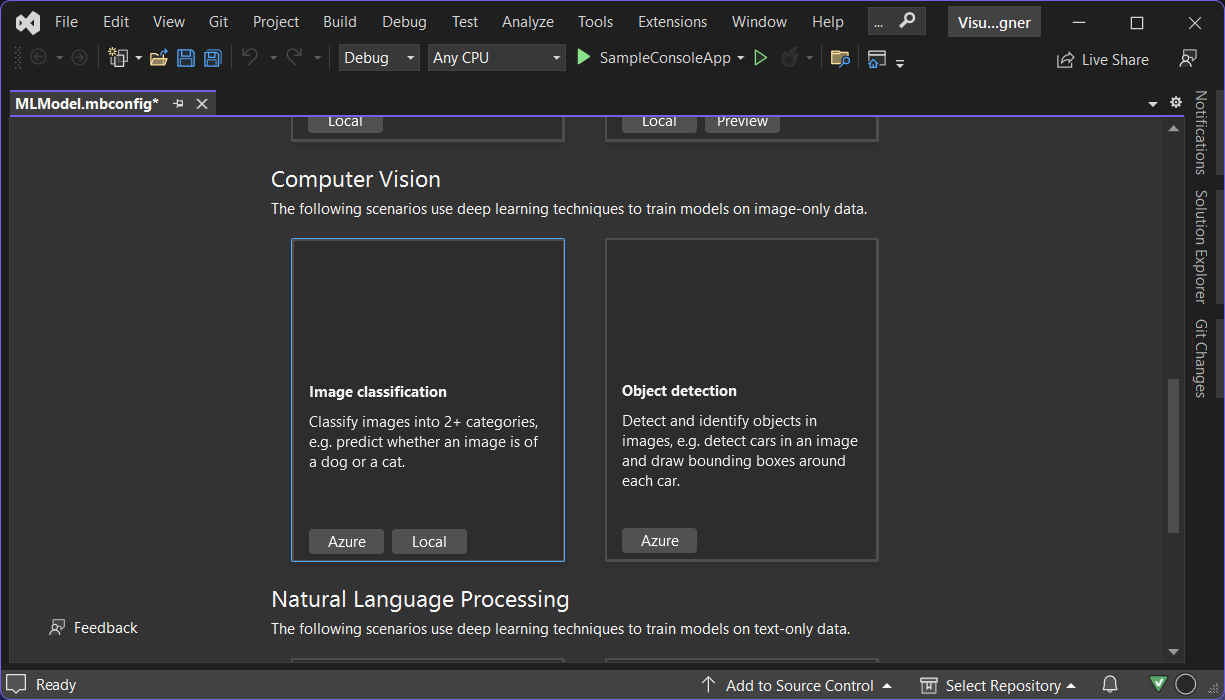
\includegraphics[width=\textwidth]{ml-net-model-builder-1-scenario}
  \caption{Zrzut ekranu ze środowiska Visual Studio pokazujący wybór scenariusza uczenia maszynowe w \emph{ML.NET Model Builder}}
  \label{fig:ml-net-model-builder-1-scenario}
\end{figure}

Takim pierwszym krokiem jest wybranie scenariusza uczenia maszynowego, które chcemy przeprowadzić w dla którego modelu chcemy wytrenować.
Wygląd takiego okna przedstawia \hyperref[fig:ml-net-model-builder-1-scenario]{rysunek \ref*{fig:ml-net-model-builder-1-scenario}}.
Do wyboru jest 7 scenariuszy z 3 większych kategorii dedykowanych pod różne zadania:

\begin{itemize}

  \item Kategoria \emph{Tabular data} -- dane tabelaryczne, czyli dane numeryczne lub tekstowe przedstawione w postaci tabeli, najczęściej w formacie CSV.
        Scenariusze w tej kategorii:

        \begin{itemize}

          \item \emph{Data classification} -- Klasyfikacja danych, służy do podziału danych na kategorie.
                Może to być klasyfikacja binarna lub wieloklasowa.
                Przykładowo klasyfikacja danych z popularnego zbioru o irysach, który na podstawie długości i szerokości płatka i działki kwiatu klasyfikuje obiekt jako jeden z trzech gatunków irysa.

          \item \emph{Value prediction} -- Przewidywanie wartości, wchodzi w zakres zadania regresji.
                Służy do przewidywania przyszłych wartości liczbowych na podstawie danych historycznych.
                Przykładowo przewidywanie ceny mieszkania na podstawie jego powierzchni i lokalizacji.

          \item \emph{Recommendation} -- Rekomendacja, przewiduje listę sugerowanych elementów dla konkretnej jednostki, w oparciu o to, jak podobne są jej upodobania do upodobań innych jednostek.
          Scenariusza rekomendacji można użyć, gdy masz zestaw  (użytkowników) i zestaw ``produktów'', takich jak przedmioty do zakupu, filmy, książki lub programy telewizyjne, wraz z zestawem ``ocen'' użytkowników tych produktów.

          \item \emph{Forecasting} -- Prognozowanie, wykorzystuje dane historyczne z szeregiem czasowym lub składnikiem sezonowym w celu na przykład przewidywania popytu lub sprzedaży produktu.

        \end{itemize}

  \item Kategoria \emph{Computer Vision} -- widzenie komputerowe, czyli przetwarzanie obrazów i wideo.
        Scenariusze w tej kategorii:
        \begin{itemize}

          \item \emph{Image classification} -- Klasyfikacja obrazów, służy do identyfikacji obrazów różnych kategorii.
                Na przykład różnych typów terenu, zwierząt lub wad produkcyjnych.
                Scenariusza klasyfikacji obrazów można użyć, jeśli masz zestaw obrazów i chcesz zaklasyfikować obrazy do różnych kategorii.

          \item \emph{Object detection} -- Wykrywanie obiektów służy do lokalizowania i kategoryzowania podmiotów na obrazach.
          Na przykład lokalizowanie i identyfikowanie samochodów i osób na obrazie.
          Wykrywania obiektów można używać, gdy obrazy zawierają wiele obiektów różnych typów.

        \end{itemize}

  \item Kategoria \emph{Natural Language Processing} -- przetwarzanie języka naturalnego, czyli analiza i generowanie tekstu.
        Scenariusze w tej kategorii:

        \begin{itemize}

          \item \emph{Text classification} -- Klasyfikacja tekstu, kategoryzuje surowy tekst wejściowy.
          Scenariusza klasyfikacji tekstu można użyć, jeśli masz zestaw dokumentów lub komentarzy i chcesz sklasyfikować je w różnych kategoriach.

        \end{itemize}

\end{itemize}

W przypadku problemu badawczego tej pracy najlepiej sprawdzi się scenariusz \emph{Image classification}, ponieważ detekcja choroby Alzheimera i stopnia demencji dążyć będzie do zaklasyfikowania obrazów mózgu do jednej z kilku kategorii, w zależności od tego, czy dany obraz jest zdrowego mózgu lub z demencją w jednym z kilku określonych stopni zaawansowania.

Po wybraniu scenariusza testowego Model Builder przekierowuje dalej do wyboru środowiska, na którym uczony będzie model.
W przypadku scenariusza \emph{Image classification} dostępne są trzy opcje: uczenie lokalne na maszynie z użyciem procesora (\emph{Local (CPU)}), uczenie lokalne z użyciem procesora graficznego (\emph{Local (GPU)}) oraz uczenie z wykorzystaniem środowiska chmurowego \emph{Azure}.
Te ostatnie możliwe jest do przeprowadzenia tylko dla scenariuszy klasyfikacji obrazów oraz wykrywania obiektów.
Co ciekawe scenariusz wykrywania obiektów można przeprowadzić wyłacznie w chmurze, lokalne uczenie nie jest możliwe.
Poza nim wszystkie pozostałe scenariusze pozwalają na uczenie przy użyciu lokalnego procesora CPU.
Natomiast na uczenie z użyciem procesora graficznego GPU jest dostępne tylko dla scenariuszy klasyfikacji obrazów oraz klasyfikacji tekstu.
Dodatkowo wymaganiem do jego przeprowadzenia jest zgodność procesora graficznego z technologią CUDA oraz zainstalowany zestaw narzędzi CUDA wersji $10.1$ oraz bibliotekę akceleracji sprzętowego \emph{CUDA Deep Neural Network} (\emph{cuDNN}) w wersji $7.6.4$.
Ważne jest, aby zainstalowana wersja była dokładnie tą sugerowaną -- niższa, a także nawet wyższa poskutkuje brakiem możliwości przeprowadzeni uczenia z użyciem lokalnego procesora graficznego.

W celu przeprowadzenia uczenia lokalnie w jak najkrótszym czasie najlepiej jest wybrać opcję \emph{Local (GPU)}.

Po wybraniu środowiska Model Builder prosi o wybranie zbioru danych uczących.
W przypadku scenariusza \emph{Image classification} Model Builder wymaga podania ścieżki do folderu, w którym znajdują się dane uczące.
W folderze tym powinny znajdować się podfoldery, których nazwy będą odpowiadały klasom / kategoriom, do których należą obrazy w nich zawarte.
W podfolderach tych powinny znajdować się obrazy w formacie \emph{.jpg}, \emph{.png} lub \emph{.bmp}.

Przykład tego, jak wybór zbioru danych testowych wygląda znajduje się na zrzucie ekranu przedstawionym na \hyperref[fig:ml-net-model-builder-2-training-data]{rysunku \ref*{fig:ml-net-model-builder-2-training-data}}.

\begin{figure}[ht]
  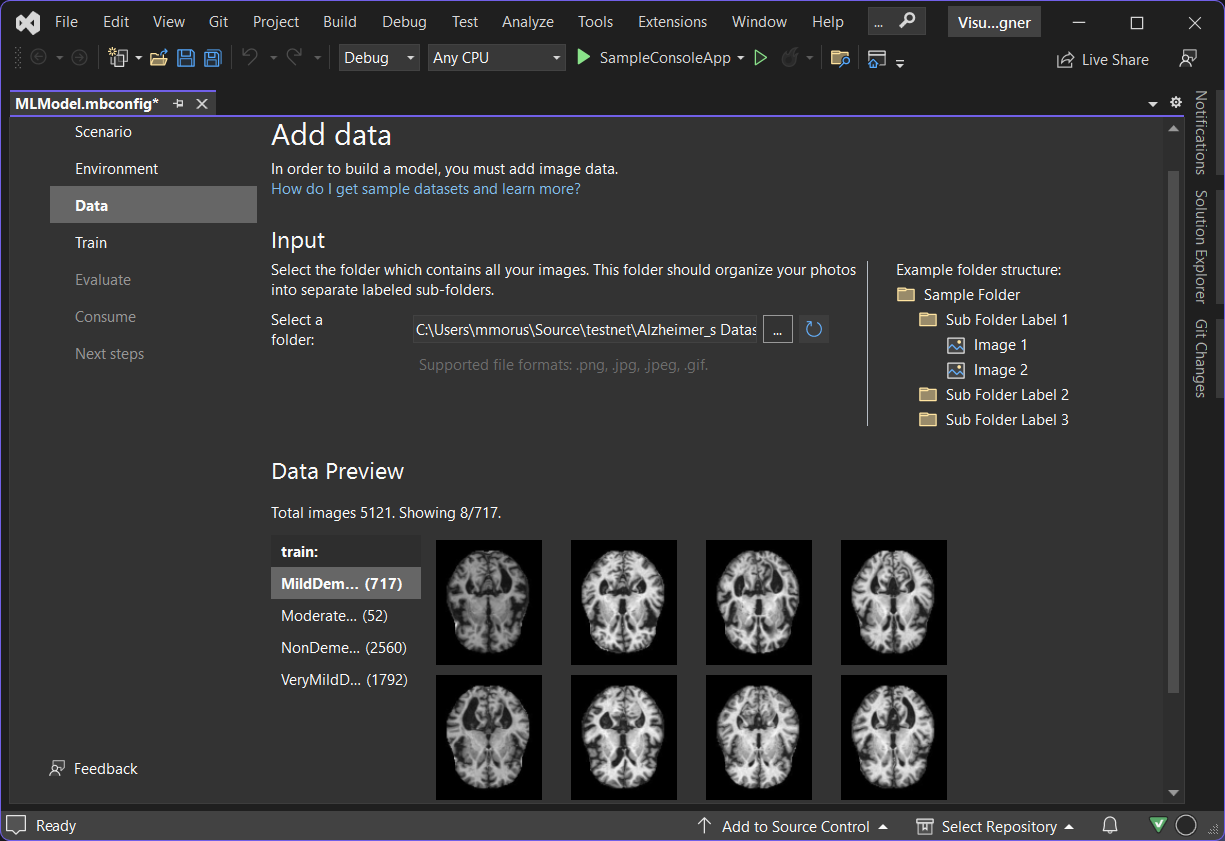
\includegraphics[width=\textwidth]{ml-net-model-builder-2-training-data}
  \caption{Zrzut ekranu ze środowiska Visual Studio pokazujący wybór danych uczących w \emph{ML.NET Model Builder}}
  \label{fig:ml-net-model-builder-2-training-data}
\end{figure}

Model Builder po wczytaniu danych przedstawia też wykryte klasy / kategorie, ilość obrazów w każdej nich oraz zsumowanych razem.
Wyświetla także przykładowe 8 z nich, tak, aby użytkownik mógł zweryfikować, czy dane zostały poprawnie wczytane oraz co się w nich znajduje.

Z opcji konfiguracyjnych Model Builder pozwala jeszcze wyłącznie na wybór jednej z czterech metryk -- mikro-dokładność (ang. \emph{micro-accuracy}), makro-dokładność (ang. \emph{macro-accuracy}), strata logarytmiczna (ang. \emph{log-loss}) lub logarytmiczna redukcja strat (ang. \emph{log-loss reduction}).
Więcej opcji konfiguracyjnych uczenie Model Builder nie posiada, użytkownik nie ma kontroli nad liczbą epok, wielkością paczki danych czy współczynnikiem uczenia -- te hiperparametry dobierane są automatycznie przez Model Builder.
Podział danych na zbiór uczący, testowy oraz walidacyjny jest również dokonywany automatycznie.

Bezpośrednio po wybraniu zbioru danych testowych rozpoczyna się uczenie faktyczne, którego postęp jest wyświetlany we wbudowanym terminalu środowiska Visual Studio oraz zapisywany jest również do pliku logów.

Po zakończeniu uczenia Model Builder wyświetla podsumowanie, które zawiera informacje o dokładności wybranej metryki modelu na zbiorze testowym oraz czasie uczenia.
Ekran podsumowujący pozwala też dodać do otwartej solucji przykładowy projekt z wykorzystaniem wytrenowanego modelu, który można wykorzystać do testów lub dalszego rozwoju.
Wygenerowany projekt posiada plik o rozszerzeniu \emph{.mlnet}, który zawiera definicję modelu i sam wytrenowany model.
Pozwala to na łatwe wykorzystanie modelu w innych projektach bez konieczności ponownego przeprowadzania uczenia.
Dodatkowo wygenerowane zostały pliki \emph{.consumption.cs} oraz \emph{.training.cs}, które zawierają kod w języku C\# odpowiednio do konsumpcji modelu oraz do jego ponownego uczenia.
Pozostałe wygenerowane pliki są zgodne z typem wybranej przykładowej aplikacji, na przykład projekt WebApi pozwalający na wykorzystanie modelu w aplikacji REST API lub projekt konsolowy pozwalający na wykorzystanie modelu z poziomu aplikacji konsolowej.

\section{Biblioteka TensorFlow.NET}
\label{sec:tensorflownet}

\emph{TensorFlow.NET} jest biblioteką do uczenia maszynowego i głębokiego uczenia maszynowego dla platformy .NET i języka C\#.
Jest to port biblioteki TensorFlow, która jest jedną z najpopularniejszych bibliotek uczenia maszynowego i głębokiego uczenia maszynowego na świecie omówionej dokładniej w \hyperref[sec:tensorflow-and-keras]{sekcji \ref*{sec:tensorflow-and-keras}}.

Ten port do platformy \emph{.NET} całkowicie omija najpopularniejszy sposób wykorzystywania biblioteki TensorFlow, czyli poprzez język Python.
Niektóre bowiem biblioteki nakładkowe w .NET dające dostęp do TensorFlow wykorzystują Pythona jako warstwę pośrednią, co powoduje konieczność instalacji Pythona i biblioteki TensorFlow wraz z wszystkimi jej zależnościami.
\emph{TensorFlow.NET} natomiast posiada powiązania bezpośrednio do kodu \emph{C} bibliotek TensorFlow, co pozwala na wykorzystanie ich w języku C\# bez konieczności instalacji Pythona oraz z maksymalną możliwą wydajność.

Projekt jest rozwijany przez społeczność programistów i jest dostępny na licencji \emph{Apache 2.0} na portalu GitHub \cite{scisharp-tensorflownet-repo}.
Jest on również częścią szerszego ekosystemu \emph{SciSharp}, który jest zbiorem bibliotek przeznaczonych do zadań z dziedziny Data Science i inżynierii danych dla platformy .NET.
W jego skład wchodzą też porty innych, bardzo popularnych bibliotek języka Python, takie jak NumSharp (port NumPy), Pandas.NET (port Pandas) czy SharpCV (port OpenCV).

W przeciwieństwie do \emph{ML.NET}, \emph{TensorFlow.NET} nie jest frameworkiem uczenia maszynowego, a biblioteką, która pozwala na wykorzystanie nie tylko gotowych modeli uczenia maszynowego i głębokiego uczenia maszynowego, ale także na tworzenie własnych modeli.
Udostępnia ona prawie wszystkie możliwości biblioteki TensorFlow, a co za tym idzie także możliwość jawnego definiowania struktury modelu uczenia maszynowego, wraz jego warstwami i parametrami.
Jest to szczególnie ważne w przypadkach, gdzie problem badawczy jest nietypowy lub nieco trudniejszy, gdzie modele oparte na uczeniu transferowym lub inne uniwersalne i tylko dostrajane rozwiązania mogą nie wystarczyć.

\emph{TensorFlow.NET} stanowi więc bardzo dobry wybór dla programistów, którzy chcą wykorzystać uczenie maszynowe w swoich projektach, ale nie chcą ograniczać się do gotowych rozwiązań, a chcą mieć pełną kontrolę nad tworzonym modelem.
Port oparty bezpośrednio na kodzie C jest bardzo wydajnym rozwiązaniem pozwalającym wykorzystać istniejące a także zbudować nowe modele uczenia maszynowego i głębokiego uczenia maszynowego działające w środowisku \emph{.NET}.
Co więcej możliwe jest użycie tej biblioteki do wytrenowanie wysoce zoptymalizowanego modelu, zapisanie go w dowolnym formacie obsługiwanym także przez TensorFlow (przykładowo \emph{ONNX}, \emph{SavedModel} czy \emph{HDF5}) i wykorzystanie wczytanie go zarówno w innych językach oprogramowania, jak także chociażby przez projekt wykorzystujący ML.NET, który jest nieco lepiej przystosowany do wykorzystania w produkcyjnych aplikacjach.

Spokrewniona biblioteka \emph{TensorFlow.Keras} jest rozszerzeniem biblioteki \emph{TensorFlow.NET}, które pozwala na tworzenie modeli uczenia maszynowego i głębokiego uczenia maszynowego w sposób bardziej wysokopoziomowy, wykorzystując do tego celu warstwy i modele z biblioteki \emph{Keras}.
Podobnie jak \emph{TensorFlow.NET}, \emph{TensorFlow.Keras} jest portem biblioteki \emph{Keras}, która jest jedną z najpopularniejszych bibliotek uczenia maszynowego i głębokiego uczenia maszynowego na świecie omówionej dokładniej w \hyperref[sec:tensorflow-and-keras]{sekcji \ref*{sec:tensorflow-and-keras}}.
Pozwala na prostsze tworzenie modeli, które są bardziej czytelne i łatwiejsze do zrozumienia, a także na wykorzystanie gotowych modeli z biblioteki \emph{Keras}.
Z tego powodu też, podobnie jak \emph{Keras} jest najczęstszym sposobem wykorzystania biblioteki \emph{TensorFlow} w warunkach rzeczywistych, tak \emph{TensorFlow.Keras} jest najczęstszym sposobem wykorzystania biblioteki \emph{TensorFlow.NET}.
